\section{Interpretations in simplified dark matter scenarios}
\label{sec:htoinv_dark_matter_models}

The results of the analysis fail to observe the Higgs boson to invisible state process, with an upper limit on the branching ratio of almost 300 times that of the \acrlong{sm}. However, limits on certain properties of dark matter may be set. One \acrshort{bsm} interpretation is presented on a Higgs portal model where the \acrshort{sm} acts as the mediator.


%=========================================================


\subsection{Higgs portal model with the standard model Higgs boson}
\label{subsec:htoinv_dark_matter_higgs_portal}

One interpretation of our results may be in terms of a simplified Higgs portal model---coupling the dark sector to the visible where the \acrshort{sm} Higgs boson acts as the mediator bridging them. An effective field theory approach assumes that the invisible decays of the Higgs boson results in the pair production of dark matter particles \Pqdark, with a frequency constrained by the upper limit on $\BRof{\higgstoinv}$. If $\mqdark < m_{\PH}/\text{2}$, on-shell production allows the translation of the \higgstoinv width $\Gamma_{\mathrm{inv.}}$ into the spin-independent $\Pqdark$-nucleon scattering cross section \xsecSI, as in Ref.~\citenum{Djouadi:2011aa}. The interaction between dark and baryonic matter may be mediated by a Higgs boson, making direct detection experiments particularly sensitive to the recoil. The sensitivity of these experiments is typically parametrised by \xsecSI as a function of dark matter mass $\mqdark$. Comparisons can therefore be made between direct detection and collider experiments.

In this Higgs portal model, two cases are considered: the dark matter candidate is a scalar, or a Majorana fermion. The branching ratio is $\BRof{\higgstoinv} = \Gamma_{\mathrm{inv.}}/(\Gamma_{\mathrm{SM}} + \Gamma_{\mathrm{inv.}})$, where we assume $\Gamma_{\mathrm{SM}} = \text{4.07}\MeV$~\cite{Heinemeyer:1559921}. From Ref.~\citenum{Djouadi:2011aa}, $\Gamma_{\mathrm{inv.}}$ can be calculated for scalar $\Pqdark_{S}$ and fermion dark matter $\Pqdark_{f}$ as
\begin{equation}
    \begin{aligned}
\Gamma^{\mathrm{inv.}}_{\PH \rightarrow \Pqdark_{S}\Pqdark_{S}} &= \frac{ \lambda^2_{\PH SS} v^2 \beta_S }{64\pi m_{\PH}},\\[0.5em]
\Gamma^{\mathrm{inv.}}_{\PH \rightarrow \Pqdark_{f}\Pqdark_{f}} &= \frac{ \lambda^2_{\PH ff} v^2 m_{\PH} \beta_f^3 }{ 32\pi \Lambda^2 }
    \end{aligned}
\end{equation}

where $\lambda$ is the coupling (scaled by $\Lambda$ in the case of fermions)\footnote{Is $\Lambda$ some sort of scale, similar to $\Lambda_{\mathrm{QCD}}$?}, $v$ is the vacuum expectation value of the \acrshort{sm} Higgs field, and $\beta_i = \sqrt{1 - 4m_{\Pqdark_i}^2/m_{\PH}^2}$. The masses of the dark matter particles $\mqdark$ are the physical masses after electroweak symmetry breaking with this new Higgs field. The spin-independent $\Pqdark$-nucleon scattering cross sections are
\begin{equation}
    \begin{aligned}
\sigma^{\mathrm{SI}}_{\Pqdark_{S}-N} &= \frac{\lambda^2_{\PH SS} }{ 16 \pi m_{\PH}^4} \frac{ m_N^4 f_N^2 }{ (m_{\Pqdark_{S}} + m_N)^2 },\\[0.5em]
\sigma^{\mathrm{SI}}_{\Pqdark_{f}-N} &= \frac{\lambda^2_{\PH ff} }{ 4 \pi \Lambda^2 m_{\PH}^4} \frac{ m_N^4 m_{\Pqdark_{f}}^2 f_N^2 }{ (m_{\Pqdark_{f}} + m_N)^2 }
    \end{aligned}
\end{equation}

where $f_N$ parametrises the Higgs-nucleon coupling. The value $f_N = \text{0.308} \pm \text{0.018}$ is taken from Ref.~\citenum{Hoferichter:2017olk}, recommended over that proposed in Ref.~\citenum{Djouadi:2011aa}. Limits on these cross sections as a function of dark matter mass are displayed in Fig.~\ref{fig:higgs_portal_dm_limits}, computed at 90\,\% confidence level to compare with direct detection experiments, whose latest results are also presented.

\begin{figure}
    \centering
    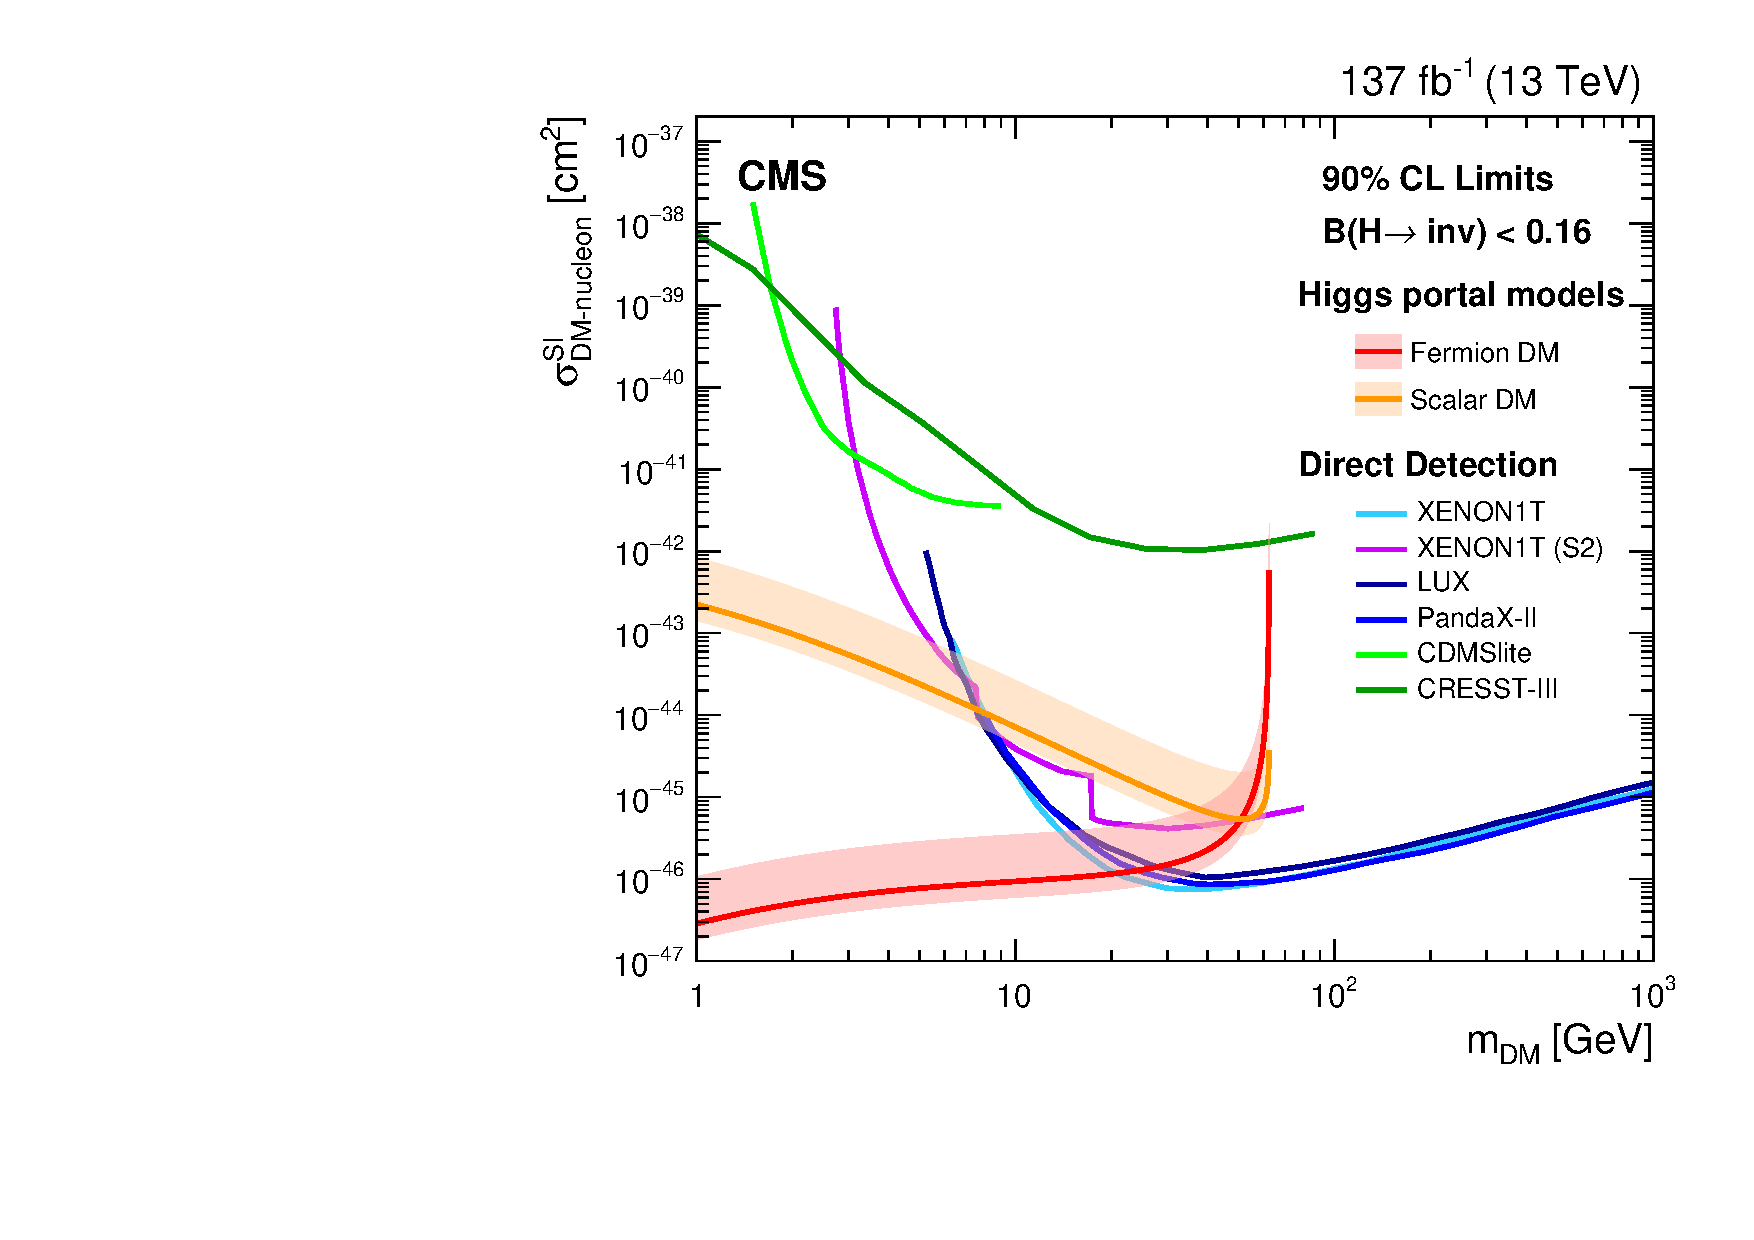
\includegraphics[width=0.6\textwidth]{figures/dark_matter_limit/higgsPortalDM.pdf}
    \caption[90\,\% confidence level upper limits on the spin-independent dark matter-nucleon scattering cross section in Higgs portal models, where the standard model Higgs boson decays into a pair of scalar (solid orange) or fermion (dashed red) dark matter particles]{90\,\% confidence level upper limits on the spin-independent dark matter-nucleon scattering cross section in Higgs portal models, where the \acrlong{sm} Higgs boson decays into a pair of scalar (solid orange) or fermion (dashed red) dark matter particles. Comparisons to direct detection experiments are also provided: XENON1T~\cite{Aprile:2018dbl} (additionally with the S2-only analysis~\cite{Aprile:2019xxb}), LUX~\cite{Akerib:2016vxi}, PandaX-II~\cite{Cui:2017nnn}, CDMSlite~\cite{Agnese:2018gze}, and CRESST-III~\cite{Abdelhameed:2019hmk}.}
    \label{fig:higgs_portal_dm_limits}
\end{figure}

For $\BRof{\higgstoinv} < \text{24\,\%}$ observed with a 90\,\% confidence level, the Higgs portal models assuming scalar and fermion dark matter candidates set the lowest limits on \xsecSI for \mqdark below 7 and 15\GeV, respectively.
